\documentclass{article}
\usepackage{graphicx}
\usepackage{amsmath}
\usepackage{amsfonts}
\usepackage[english]{babel}

\title{Multiplicitivity of Natural Numbers}
\author{Alessio Branda}
\date{September 2026}

\begin{document}

\maketitle

\section{Introduction}
The natural numbers admit many classical classifications, most notably the distinction between prime and composite numbers.

In this work, we investigate the structural patterns formed by divisibility over finite sets of initial prime numbers. Formally, we evaluate the restricted prime indicator function $\omega_S(n)$ \cite{hardyramanujan1917} over the set of the first $k$ prime numbers $S_k = \{p_1, p_2, \dots, p_k\}$. This evaluation induces a discrete invariant that we term \textit{\textbf{multiplicitivity}}, denoted $\mu_k(n)$, which counts how many fundamental primes in $S_k$ divide $n$. Because $\mu_k(n)$ depends strictly on divisibility by factors of the $k$-th primorial $P_k = p_k\# = \prod_{i=1}^k p_i$, it projects the infinite domain of natural numbers onto a finite, highly structured partition. To make this partition intuitive and visually accessible, we focus primarily on the case $k=4$, where $S_4 = \{2, 3, 5, 7\}$ and $P_4 = 210$. Within this domain, multiplicitivity partitions the integers into six discrete classes: Unico ($\mu=0$), Monome ($\mu=1$), Duome ($\mu=2$), Triome ($\mu=3$), Quadrome ($\mu=4$), and Pentanome ($\mu=5$). Through empirical visual analysis and formal modular arithmetic, we prove that this structural partition exhibits strict periodicity with period $P_4 = 210$ and reflection symmetry centered at $P_4/2 = 105$. Finally, we demonstrate how this framework generalizes naturally to arbitrary $k$-th primorials $P_k$, connecting our empirical taxonomy directly to classical primorial residue systems.

Throughout the paper, the natural numbers domain is defined as $\mathbb{N}=\mathbb{Z^+}$.

\section{Classification of natural numbers}
Let us start by defining the foundation block of the whole paper: \textit{\textbf{fundamental numbers}} are the combination of the number 1 and the first 4 prime numbers:
$$
\mathbb{F} = \{1, 2, 3, 5, 7\}.
$$
From this we then defined a new classification for the numbers. Assume $n\in\mathbb{N}\setminus \mathbb{F}$, then:
\begin{itemize}
    \item if $n$ is divisible by only one of the fundamental numbers, then it is defined as a \textit{\textbf{monome}};
    \item if $n$ is divisible by only two of the fundamental numbers, then it is defined as a \textit{\textbf{duome}};
    \item if $n$ is divisible by only three of the fundamental numbers, then it is defined as a \textit{\textbf{triome}};
    \item if $n$ is divisible by only four of the fundamental numbers, then it is defined as a \textit{\textbf{quadrome}};
    \item if $n$ is divisible by only five of the fundamental numbers, then it is defined as a \textit{\textbf{pentanome}};
\end{itemize}
Let us now, however, make some observations: for these classifications, the fundamental numbers were not included since we need to apply a rule:
\paragraph{Rule of fundamental numbers} Every fundamental prime $p \in \{2,3,5,7\} $ is classified as a monome, since its only fundamental divisor is 1.

As an example of the rule, let us take the number 2: it can be decomposed only as $2 = 1\cdot 2$, but $2\in \mathbb{F}$, therefore its only fundamental divisor is 1, so it is a \textit{monome}. Such concept will become clearer once we introduce a new characteristic of natural numbers: \textit{\textbf{multiplicitivity}}.

\section{Multiplicitivity of natural numbers}
We define the \textbf{\textit{multiplicitivity}} of a natural number as follows.

Multiplicitivity $\mu$ is the number of fundamental numbers that make the baseline of the number disregarding the number itself, otherwise one could argue that every number has $\mu = 1$ since $x = 1\cdot x$.

For visualization, let us provide three example:
\begin{itemize}
    \item $32 = 1\cdot 2^5 \rightarrow \mu(32)=2$
    \item $474 = 1\cdot 2\cdot3\cdot 79 \rightarrow\mu(474)=3$
    \item An interesting case is $p\in\mathbb{F}$: let us see each case
    \begin{itemize}
        \item The number 1 is the most special case: it is an \textit{\textbf{unico}}: an unico is a number of multiplicitivity of 0. Let us remember that the multiplicitivity is the count of fundamental numbers that make up the number without counting the number itself, so what happens when the number itself is also the only fundamental number it is made up of? Then: $$\mu(1)=0.$$
        \item Given $p'\in\mathbb{F}\setminus\{1\}$:
        $$    \mu(p')=1.
        $$
    \end{itemize}
    For this case, we define the \textit{\textbf{fundamental primes}} as $$\mathbb{P}=\{2,3,5,7\}.$$
\end{itemize}
Without this distinction, a prime like $2$ would have two divisors in $\mathbb{F} = \{1, 2, 3, 5, 7\}$ (namely $1$ and $2$), making it a duome, while any prime $p \ge 11$ would only have $1$ as a fundamental divisor, making it a monome. By explicitly treating the baseline divisor $1$ and fundamental primes systematically, we guarantee that all prime numbers without exception share the uniform classification of monome ($\mu = 1$).


Mathematically, we define the multiplicitivity $\mu(n)$ of a natural number $n \in \mathbb{N}$ as:
\[
\mu(n) = \#\{p \in \mathbb{F} : p \mid n\} - \#(\{n\} \cap \mathbb{F})
\]
or equivalently,
\[
\mu(n) = \#\{p \in \mathbb{F} : p \mid n\} - \mathbf{1}_{\mathbb{F}}(n)
\]
where $\mathbb{F} = \{1, 2, 3, 5, 7\}$.

We can then classify natural number as shown in Table \ref{tab:classes}.

\begin{table}[h!]
    \centering
    \begin{tabular}{c|c}
        Multiplicitivity $\mu$ & Class  \\
        \hline
        0 & Unico \\
        1 & Monome \\
        2 & Duome \\
        3 & Triome \\
        4 & Quadrome \\
        5 & Pentanome
    \end{tabular}
    \caption{Classes of natural numbers with regard to their multiplicitivity.}
    \label{tab:classes}
\end{table}

This imposes that a natural number can be represented as:
$$
n = 1\cdot2^{\delta_n}\cdot 3^{\tau_n} \cdot 5^{\pi_n} \cdot 7^{\epsilon_n} \cdot \xi 
$$
where $\xi$ is a non-fundamental prime factor and it does not affect multiplicitivity and can even be an unico.

\section{Empirical observations}
The best way to work with numbers is to visualize them. The first step taken was to plot the histogram of the distribution of the classes (see Figure \ref{fig:dist_tot}). 
\begin{figure}[h!]
    \centering
    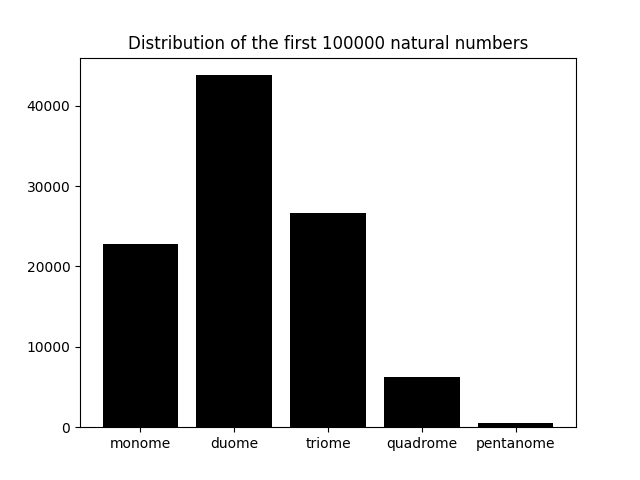
\includegraphics[width=0.875\linewidth]{figures/dist_tot.png}
    \caption{Distribution of classes for the first $10^5$ natural numbers.}
    \label{fig:dist_tot}
\end{figure}

The first pentanome encountered is \textbf{210} (and, by its definition, all the other are its multiples). This number represents a specific point that binds the concept of $\mu$.

Let us first visualize the distribution of the numbers from 1 to 210. As shown in Figure \ref{fig:dist_1_210}, the distribution follows that of the overall group of numbers: this suggests that the pentanome may represent a point of periodicity.

\begin{figure}[h!]
    \centering
    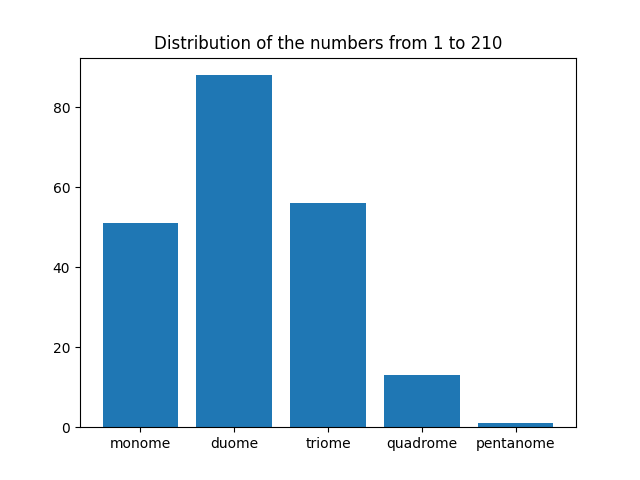
\includegraphics[width=0.75\linewidth]{figures/dist_1_210.png}
    \caption{Distribution of classes for the numbers from 1 to 210.}
    \label{fig:dist_1_210}
\end{figure}
Empirically, such pattern shows, in fact in Figure \ref{fig:dist_ranges} one can see that ranges of pentanome multiples follow the same distribution, apart from the overall overshooting of the monome population in the initial range to the fundamental prime population.
\begin{figure}[h!]
    \centering
    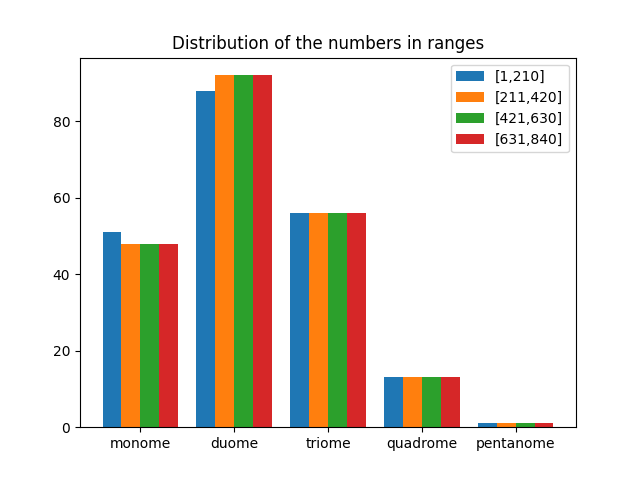
\includegraphics[width=0.75\linewidth]{figures/dist_ranges.png}
    \caption{Distribution of classes for numbers in ranges of 210.}
    \label{fig:dist_ranges}
\end{figure}
Let us now look at this pattern. In Figure \ref{fig:mult_2000} is shown the plot of the multiplicitivity for each number from 1 to 2000.

\begin{figure}[h!]
    \centering
    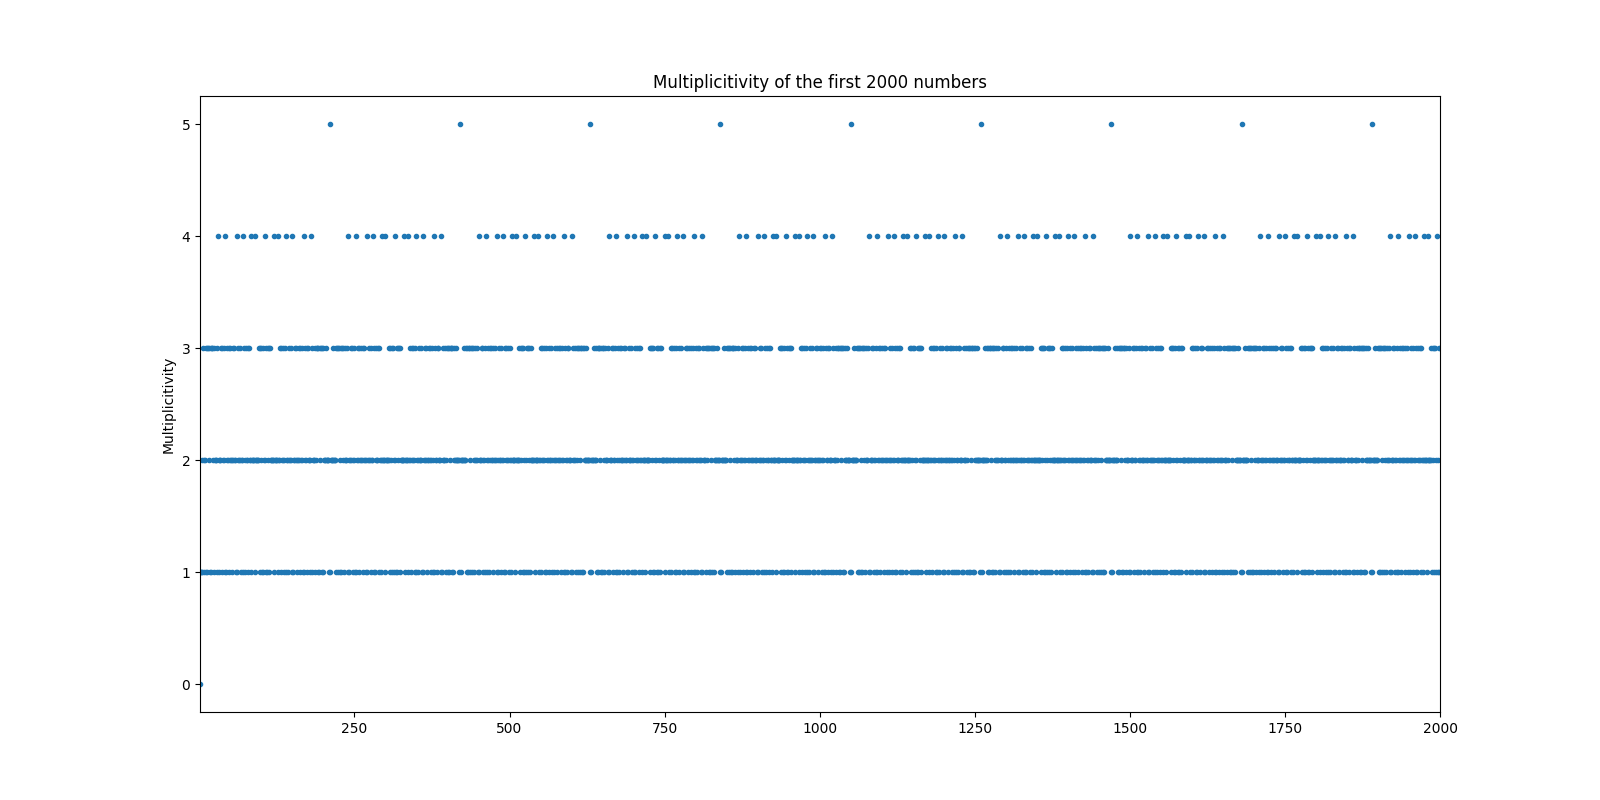
\includegraphics[width=1\linewidth]{figures/pattern.png}
    \caption{Multiplicitivity of the first 2000 numbers.}
    \label{fig:mult_2000}
\end{figure}

One can notice that after every pentanome, the pattern follows the same (apart from the first sequence) pattern: this was better visualized in Figure \ref{fig:patterns}.
\begin{figure}[h!]
    \centering
    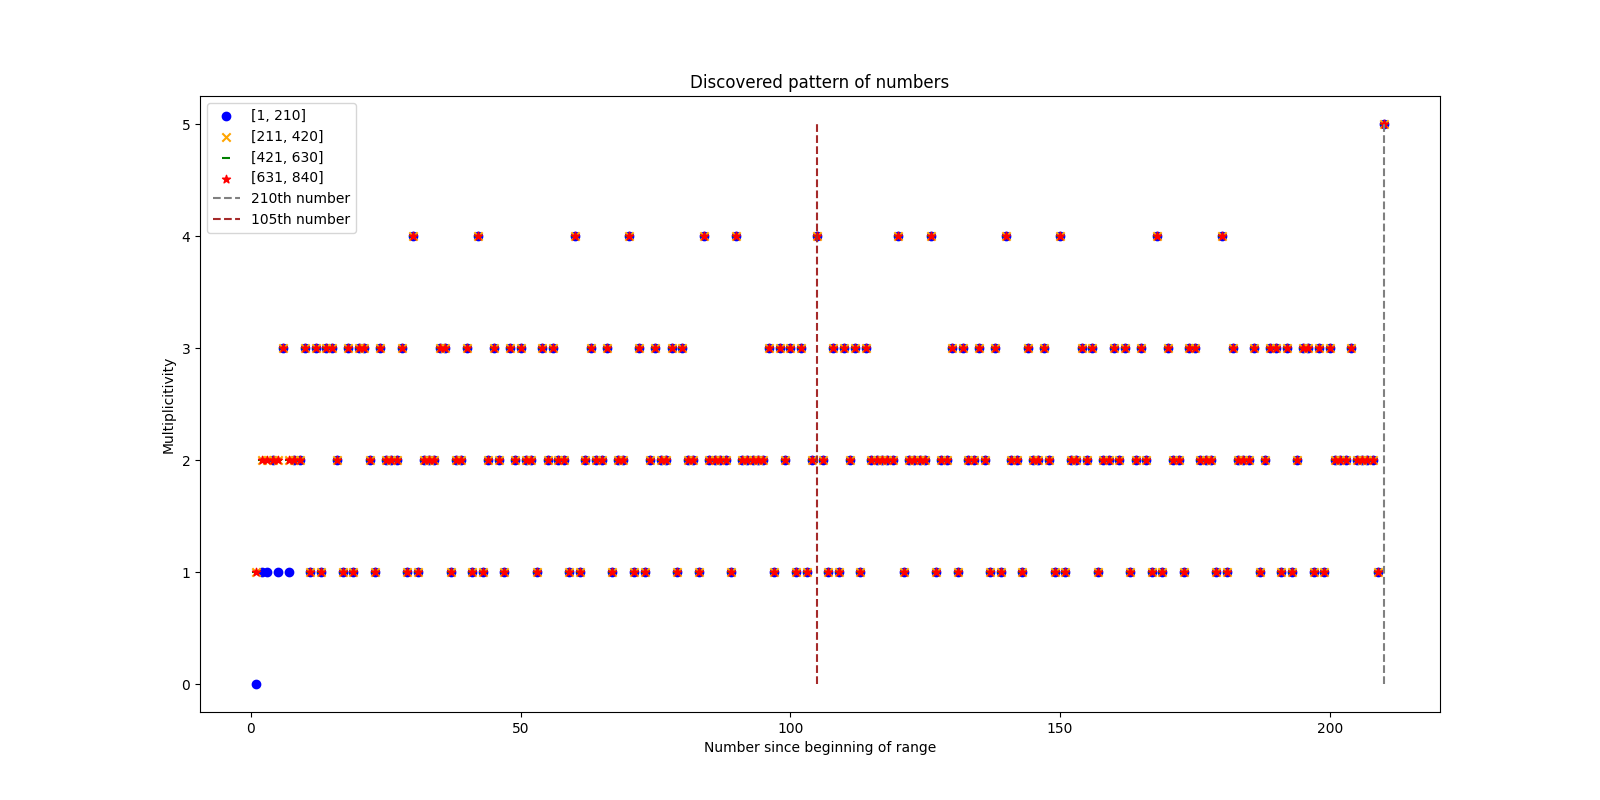
\includegraphics[width=1\linewidth]{figures/pattern_ranges.png}
    \caption{Multiplicitivity pattern of different ranges of 210 numbers.}
    \label{fig:patterns}
\end{figure}
The only difference in the sets is given by the unico and first 4 monome numbers, i.e. the fundamental numbers!
Therefore, one can formulate the following observation: \textit{after every multiple of 210, after the first set, the pattern appears to repeat itself. Since the pentanomes represent the numbers that allow for all combinations of each fundamental number, the numbers in between follow the same pattern in multiplicitivity.}


An additional observation can be made regarding the \textit{central point of the sequence}: the 105th point (meaning 210/2) represents the \textit{specular point} of the sequence. \textit{Two numbers distancing from the left as much as from the right of the 105th point, the multiplicitivity is equivalent: the pattern is specular with axes on the 105th point of the sequence.}

\section{Theorem and Lemma}
\paragraph{Theorem (Periodical Multiplicitivity)} Given a natural number $n$ not part of the fundamental numbers,
$$
\mu(n) = \mu(n+210m) \quad \forall n\in\mathbb{N} \setminus \mathbb{F}, \forall m\in\mathbb{N}
$$
i.e. the multiples of 210 are the \textit{\textbf{pentanomes}} and represent the \textit{periodic points} of natural numbers.

The restriction $n \notin \mathbb{F}$ is required specifically because the fundamental primes $p \in \{2, 3, 5, 7\}$ are assigned $\mu(p) = 1$ by rule (disregarding themselves as prime factors), whereas their shifted counterparts $p + 210m$ are evaluated standardly by their full set of fundamental factors.

\paragraph{Lemma (Specular Quadrome)} Given a natural number $k$ in the range \{1, ..., 104\},
$$
\mu(105 (1+2m)+ k)=\mu(105 (1+2m) - k)    \quad \forall m\in \mathbb{N}, k \in \{1, 2, \dots, 104\}
$$
i.e. the odd multiples of 105 are the \textit{\textbf{specular quadromes}} and represent the points in which, within each sequence of the 210th numbers, the multiplicitivity pattern becomes symmetric.

\subsection{Proofs}
\paragraph{Theorem} Given $n\in \mathbb{N} \setminus \mathbb{F}, p\in\mathbb{F}$:
$$
n+210=n+(1\cdot2\cdot 3 \cdot 5 \cdot 7)
$$
therefore, we want to prove that:
$$
p|n\Leftrightarrow p|(n+210)
$$
Let us start by proving that if $p|n$, then $p|(n+210)$; let us define
\begin{align*}
n &= a\cdot p \quad \forall a\in\mathbb{N} \\
210 &= b\cdot p \quad \forall b\in\mathbb{N}
\end{align*}
therefore,
$$
n+210=ap+bp=(a+b)p
$$
$$ \Rightarrow p|(n+210). $$
Now we want to prove that if $p|(n+210)$, then $p|n$; let us define 
\begin{align*}
n + 210 &= c\cdot p \quad \forall c\in\mathbb{N} \\
210 &= b\cdot p \quad \forall b\in\mathbb{N}
\end{align*}

$$
n = n+210-210=cp-bp = (c-b)p \equiv ap
$$
$$ \Rightarrow p|n. $$
Since the argument works for $n\rightarrow n+210$, by induction it holds for all multiples $210m$. Q.E.D.

\paragraph{Lemma}
Let us define
$$
N^+ = 105(1+2m)+k= 105+210m+k,
$$
$$
N^-=105(1+2m)-k=105+210m-k.
$$
We need to demonstrate that for each fundamental number $p\in\mathbb{F}$,
$$
p|N^+ \Leftrightarrow p|N^-
$$
\begin{itemize}
    \item $p=1$: this is trivial since 1 divides every integer, so it contributes equally to both sides;
    \item $p\in\{3,5,7\}$: note that $105 = 3\cdot 5\cdot 7$, so:
    $$
    105 \equiv 0 \pmod p \text{ for } p\in\{3,5,7\}
    $$ 
    and $210m\equiv 0 \pmod p$ as well.
    
    Thus:
    $$
    N^+ \equiv k \pmod p, \quad N^-\equiv -k \pmod p.
    $$
    However:
    $$
    p|k \Leftrightarrow p|-k,
    $$
    therefore:
    $$
    p|N^+ \Leftrightarrow p|N^- \text{ for } p\in\{3,5,7\};
    $$
    \item $p=2$: we have:
    $$
    105 \equiv 1 \pmod 2, \quad 210m \equiv 0 \pmod 2
    $$
    meaning that
    $$
    N^+ \equiv 1+k \pmod 2, \quad N^- \equiv 1-k \pmod 2.
    $$
    Let us now notice that:
    \begin{itemize}
        \item if $k$ is even, then $1+k$ and $1-k$ are both odd, therefore neither are divisible by 2;
        \item if $k$ is odd, then $1+k$ and $1-k$ are both even, therefore both are divisible by 2.
    \end{itemize}
    This implies that:
    $$
    2|N^+ \Leftrightarrow 2|N^-.
    $$
\end{itemize}
We have found that, for every $p\in \mathbb{F}$,
$$
p|N^+ \Leftrightarrow p|N^-
$$
hence, they have the same set of fundamental divisors and, therefore:
$$
\mu(N^+) = \mu(N^-)
$$
Q.E.D.

\subsection{Examples}

We now provide explicit examples illustrating the Lemma of Specular Quadrome.
For simplicity, we fix $m = 1$, so the specular center is

\[
105(1 + 2m) = 315.
\]

For each $k \in [1,104]$, the lemma states that

\[
\mu(315 + k) = \mu(315 - k).
\]

\paragraph{Example 1: $k = 10$}

\[
\mu(325) = \mu(305).
\]

Indeed,

\[
325 = 1 \cdot 5^2 \cdot 13 \quad \Rightarrow \quad \mu(325) = 2,
\]

\[
305 = 1 \cdot 5 \cdot 61 \quad \Rightarrow \quad \mu(305) = 2.
\]

Since both numbers lie in $\mathbb{N}\setminus \mathbb{F}$, periodicity also gives

\[
\mu(325 - 210) = \mu(305 - 210).
\]

\paragraph{Example 2: $k = 23$}

\[
\mu(338) = \mu(292) = \mu(128) = \mu(82).
\]

We compute:

\[
128 = 1 \cdot 2^7 \quad \Rightarrow \quad \mu(128) = 2,
\]

\[
82 = 1 \cdot 2 \cdot 41 \quad \Rightarrow \quad \mu(82) = 2.
\]

\paragraph{Example 3: $k = 1$}

\[
\mu(316) = \mu(314) = \mu(106) = \mu(104).
\]

Indeed,

\[
106 = 1 \cdot 2 \cdot 53 \quad \Rightarrow \quad \mu(106) = 2,
\]

\[
104 = 1 \cdot 2^3 \cdot 13 \quad \Rightarrow \quad \mu(104) = 2.
\]

\paragraph{Example 4: $k = 104$}

\[
\mu(419) = \mu(211).
\]

Both numbers are monomes:

\[
419 = 1 \cdot 419 \quad \Rightarrow \quad \mu(419) = 1,
\]

\[
211 = 1 \cdot 211 \quad \Rightarrow \quad \mu(211) = 1.
\]

However, note that the symmetric pair around $105$ in the first block,

\[
209 \quad \text{and} \quad 1,
\]

does \emph{not} satisfy $\mu(209) = \mu(1)$, since

\[
\mu(209) = 1, \qquad \mu(1) = 0.
\]

This is why the lemma requires $m \geq 1$.

\subsection{Generalization to $k$-th Multiplicitivity}
The framework established for $\mathbb{F} = \{1, 2, 3, 5, 7\}$ extends naturally to larger sets of fundamental primes. We define the generalized fundamental set $\mathbb{F}_k$ as:
\[
\mathbb{F}_k = \{1\} \cup \mathbb{P}_k
\]
where $\mathbb{P}_k = \{p_1, p_2, \dots, p_k\}$ denotes the set of the first $k$ prime numbers.

For any $n \in \mathbb{N}$, the generalized multiplicitivity $\mu_k(n)$ is defined as:
\[
\mu_k(n) = \#\{p \in \mathbb{F}_k : p \mid n\} - \mathbf{1}_{\mathbb{F}_k}(n)
\]
\[
(0\leq \mu_k(n)\leq k+1)
\]

Let $\kappa = p_k\# = \prod_{i=1}^k p_i$ denote the $k$-th primorial. 

With this, prime and semiprimes still can be denoted as \textit{monomes}, however the current class classification does not generalize to arbitrary $k$. We therefore propose a \textit{generalized classification of natural numbers} as displayed in Table \ref{tab:classes_general}.

\begin{table}[h!]
    \centering
    \begin{tabular}{c|c}
        Multiplicitivity $\mu_k$ & Class  \\
        \hline
        0 & Unico \\
        1 & Monome \\
        $2 \dots k$ & $\mu_k$-ome\\
        $k+1$ & Plenome
    \end{tabular}
    \caption{Classes of natural numbers with regard to their $k$-th multiplicitivity.}
    \label{tab:classes_general}
\end{table}
As an example, if $k=7$, a number with $\mu_7=6$ (for example 30030) is a \textit{6-ome} (or \textit{hexaome}) within that specific framework.


The periodic and specular properties of multiplicitivity generalize as follows:

\paragraph{Theorem (Periodicity of $k$-th Multiplicitivity)} 
For any integer $n \in \mathbb{N} \setminus \mathbb{F}_k$ and any $m \in \mathbb{N}$,
\[
\mu_k(n) = \mu_k(n + m\kappa)
\]
That is, the generalized multiplicitivity $\mu_k(n)$ is strictly periodic with fundamental period given by the $k$-th primorial $\kappa = p_k\#$.

\paragraph{Lemma (Specular Symmetry of $k$-th Multiplicitivity)} 
For any $m \in \mathbb{N}$, $k>1$ and any offset integer $j \in \left\{1, 2, \dots, \frac{\kappa}{2} - 1\right\}$,
\[
\mu_k\left(\frac{\kappa}{2}(1 + 2m) + j\right) = \mu_k\left(\frac{\kappa}{2}(1 + 2m) - j\right)
\]
That is, within each period of length $\kappa$, the pattern of $\mu_k(n)$ exhibits reflection symmetry centered at the odd half-integer multiples of $\kappa$.

\paragraph{Proof Sketch for the Generalized Formulations}
The proofs for the generalized Periodicity Theorem and Specular Symmetry Lemma follow identically by replacing the specific prime set $\mathbb{P}_4 = \{2, 3, 5, 7\}$ and its primorial $P_4 = 210$ with $\mathbb{P}_k = \{p_1, \dots, p_k\}$ and $\kappa = p_k\#$, respectively. 


For periodicity, since $\kappa = \prod_{i=1}^k p_i$, every fundamental prime $p \in \mathbb{P}_k$ satisfies $p \mid \kappa$, yielding $n + m\kappa \equiv n \pmod p$ for all $m \in \mathbb{N}$. 


For specular symmetry around $\frac{\kappa}{2}(1 + 2m)$, odd fundamental primes $p \in \mathbb{P}_k \setminus \{2\}$ divide $\frac{\kappa}{2}$, giving $\frac{\kappa}{2}(1 + 2m) \pm j \equiv \pm j \pmod p$, while $p = 2$ reduces to parity analysis of $\frac{\kappa}{2} \pm j$ since $\kappa$ is even. 


Thus, the divisibility equivalences established in Section 5.1 hold uniformly for all $p \in \mathbb{F}_k$.

\paragraph{Corollary ($k=0$ degeneracy)} To be feasible, the definition of multiplicitivity applies to the first $k\in\mathbb{N}$ prime numbers. For $k=0$, $\mathbb{F}_0=\{1\}$ which would imply that all non-fundamental numbers are of multiplicitivity 1 and the period would be 1 itself, breaking the lemma.

\paragraph{Corollary ($k=1$ degeneracy)} For $k=1$, $\kappa$ = 2 and $\kappa$/2 - 1 = 0, so the index set \{1,...,$\kappa$/2-1\} is empty. The Lemma of Specular Symmetry therefore holds vacuously at $k=1$, asserting no non-trivial constraint. The restriction $k>1$ is imposed purely to keep the statement meaningful, not because $k=1$ violates it.


\section{Connection to Classical Number Theory}
While the definition of multiplicitivity and its associated taxonomy are novel, the underlying mechanisms governing its periodicity and symmetry are rooted in well-known number-theoretic concepts.

The period $210 = 2 \cdot 3 \cdot 5 \cdot 7$ corresponds to the fourth primorial $P_4 = p_4\# = 7\#$. In sieve theory and wheel factorization, primorials naturally define the fundamental period for divisibility patterns across initial sets of primes \cite{halberstam1974}. Any function depending solely on membership in residue classes modulo $\{2, 3, 5, 7\}$ must necessarily be periodic modulo $7\# = 210$.

Similarly, the reflection symmetry centered at $105 = 210/2$ reflects the classical property of greatest common divisors within modular systems: for any integers $a$ and $m$, $\gcd(a, m) = \gcd(m - a, m)$ \cite{hardy2008}. Applied to $m = 210$, any fundamental prime $p \in \{2, 3, 5, 7\}$ divides $105 + j$ if and only if it divides $105 - j$ (with special handling for $p=2$ via parity). 

Thus, multiplicitivity can be viewed as a concrete, bounded invariant that projects these classical primorial symmetries into a clear 6-class structural partition of $\mathbb{N}$ \cite{apostol1976}.

While formulated independently from an empirical perspective, the concept of multiplicitivity $\mu(n)$ can be formally viewed as a restricted prime factor indicator function $\omega_S(n)$ \cite{hardyramanujan1917} evaluated over the finite prime support $S = \{2, 3, 5, 7\}$. Specifically, for any $n \in \mathbb{N} \setminus \mathbb{F}$,$$\mu(n) = 1+\omega_{\{2,3,5,7\}}(n) = 1+\sum_{p \in \{2,3,5,7\}} \mathbf{1}_{p \mid n}$$
For such reason, a generalization to the $k$-th prime number was proposed, generalizing the definition of multiplicitivity and, consequently, the theorem and lemma.

\section{Conclusion}
In this work, we introduced the concept of \textit{multiplicitivity}, a discrete invariant and structural classification of natural numbers defined by divisibility over sets of fundamental prime numbers. Starting from an empirical visual analysis for $k=4$, where $\mathbb{F}_4 = \{1, 2, 3, 5, 7\}$, we showed that multiplicitivity partitions the natural numbers into six intuitive classes: Unico, Monome, Duome, Triome, Quadrome, and Pentanome. We proved that this partition exhibits strict periodicity with fundamental period $P_4 = 210$ (the first pentanome) and reflection symmetry centered at odd multiples of $P_4/2 = 105$.

We then established that this behavior is not merely an isolated arithmetic curiosity, but a concrete projection of classical primorial residue systems. By extending the framework to arbitrary $k \in \mathbb{N}$, we formalized the generalized $k$-th multiplicitivity $\mu_k(n)$ over the fundamental set $\mathbb{F}_k = \{1\} \cup \mathbb{P}_k$. We demonstrated that the corresponding periodic and specular properties scale universally to all primorials $\kappa = p_k\#$, proving that $\mu_k(n)$ acts as a bounded, highly structured indicator function $\omega_{\mathbb{P}_k}(n)$.

By bridging empirical visualization with formal modular arithmetic, multiplicitivity translates the abstract algebraic structure of $\mathbb{Z} / p_k\#\mathbb{Z}$ into an accessible, geometric taxonomy. Future research may explore the asymptotic class density distributions as $k \to \infty$, the distribution of multiplicitivity gaps between consecutive primes, and potential applications to optimizing bounded wheel factorization algorithms.

\newpage

\bibliographystyle{plain} % Options: plain, unsrt, alpha, abbrv, etc.
\bibliography{references}

\end{document}